\chapter{Lecture 19}
\section{Landau rate}
Recall from last lecture that the Nyquist-Shannon sampling theorem tells us a minimal sampling rate necessary to recover a bandlimited signal. A generalization of the Nyquist sampling rate is the Landau rate. 
\cbeqn{Landau sampling rate}{
    \txt{If } \lambda\left(supp(\mathcal{F}(f))\right) = 2M > 0 \txt{ with } \lambda=\txt{Lebesgue measure}, \txt{ then } \label{eqn:18:nyquistsampling} \\
    f \txt{ is }  \txt{recovered by samples whose maximal step size is } \Delta t = \frac{1}{2M} \nonumber
}
\askbjorn{This seems to not be the right statement based on the paper by Landau. That paper seems to restrict attention to a finite union of compact intervals.}
The Landau sampling rate thus generalizes the Nyquist sampling theorem to (a) sets whose support in Fourier domain is disconnected and (b) to nonuniform grid sampling.

\askbjorn{Go through nonuniform sampling for homogenization}

\section{Kolmogorov $n$-width in context of POD}
Let us look at how Kolmogorov $n$-width relates to POD. Let $X=\R^2$ be our normed linear space and our set $A$ to be given by
\begin{align*}
    A = \{x=(x_1,x_2)\in \R^2 : x_2 = x_1 + sin(j x_1), j \in \mathbb{N}\}.
\end{align*}
This space is illustrated in Figure \ref{fig:19:A}. This figure shows us that $A$ is a sequence of sinusoidal perturbations of the identity. In our context, our norm is simply the Euclidean norm $\|\bs{x}\|_2^{2} = x_1^2 + x_2^2$. First, we note that $d_2(A,\R^2) = 0$ because $\R^2$ is the whole space and is a $2$-dimensional subspace of itself. What is $d_1(A,\R^2)$? One-dimensional subspaces are just lines passing through the origin, i.e. sets of the form $Y_{\alpha} = span\left[(\alpha, 1)^{T}\right]$ for some $\alpha$. 
\begin{figure}
    \centering
    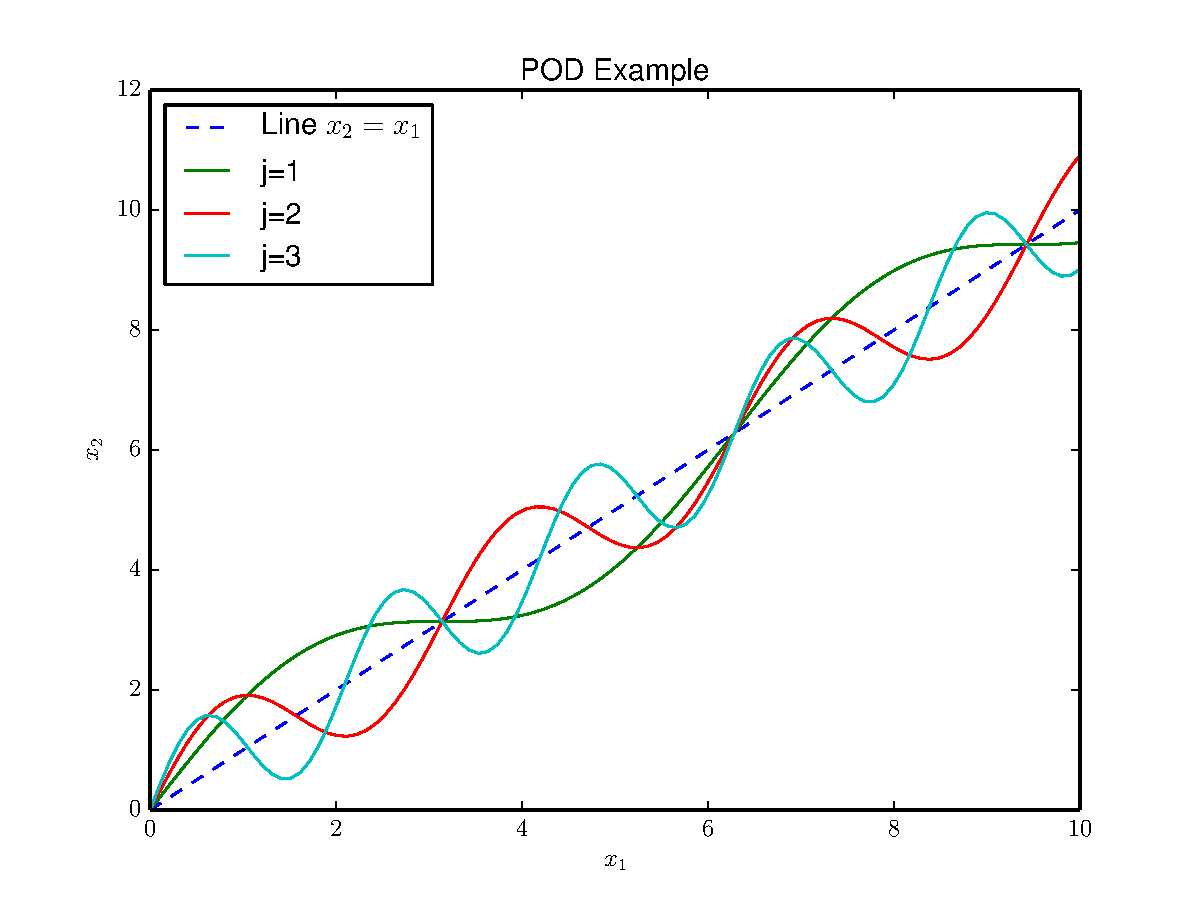
\includegraphics[width=\textwidth]{images/pod.pdf}
    \caption{Illustration of set $A$, which contains a sequence of sinusoidal perturbations of the identity.}
    \label{fig:19:A}
\end{figure}
Therefore, using the definition of Kolmogorov $1$-width, we can rewrite as
\begin{align} \label{eqn:19:kol1width}
d_1(A,\R^2) = \inf_{\alpha \in \R} \left[ \sup_{\bs{x} \in A} \left(\inf_{\bs{y} \in Y_{\alpha}} \|\bs{x}-\bs{y}\|\right)\right]
\end{align}
For $\bs{y} \in Y_{\alpha}$ and $\bs{x} \in A$, we have
\begin{align} \label{eqn:19:diff}
\|\bs{x} - \bs{y}\|^2 = (x_1 - y_1)^2 + (x_1 - \alpha y_1 + sin(j x_1))^2 := g(x_1,y_1).
\end{align}
The expression in Equation \eqref{eqn:19:kol1width} tells to first minimize over all values of $\bs{y}$ (that is, find $dist(\bs{x}, Y_{\alpha})$ first). Setting $\frac{\partial g}{\partial y_1} = 0$ and solving gives
\begin{align} \label{eqn:19:distY}
\frac{\partial g}{\partial y_1} = 0 &\Leftrightarrow y_1 = x_1 + \frac{\alpha}{1 + \alpha} sin(jx_1).
\end{align}
Plugging Equation \eqref{eqn:19:distY} into Equation \eqref{eqn:19:diff}, we arrive at
\begin{align} \label{eqn:19:inf}
\inf_{\bs{y} \in Y_{\alpha}} \|\bs{x} - \bs{y}\| = \sqrt{\frac{\alpha^2}{(1+\alpha)^2} sin^2(jx_1) + \left[ (1-\alpha)x_1 + \frac{\alpha^2 - \alpha - 1}{1+\alpha} sin(jx_1)\right]^2}
\end{align}
after taking the square root. Equation \eqref{eqn:19:kol1width} tells us that we now take a supremum over all $\bs{x} \in A$. We note that Equation \eqref{eqn:19:inf} shows us immediately that this supremum is infinite whenever $\alpha \neq 1$. The case when $\alpha=1$ reduces nicely to the expression $2^{-1/2} |sin(jx_1)|$ which takes maximal value $2^{-1/2}$. Thus we have
\begin{align}
    \sup_{\bs{x} \in A} \left( \inf_{\bs{y} \in Y_{\alpha}} \|\bs{x} - \bs{y}\|\right) = \begin{cases}
    \frac{1}{\sqrt{2}} & \alpha = 1 \\
    \infty & \alpha \neq 1
    \end{cases}
\end{align}
Our last step in Equation \eqref{eqn:19:kol1width} is take the infimum over all subspaces, i.e., over all slopes $\alpha$. This finally gives us that 
\begin{align} \label{eqn:19:kolfinal}
d_{1}(A,\R^2) = \inf_{\alpha \in \R} \left[ \sup_{\bs{x} \in A} \left( \inf_{\bs{y} \in Y_{\alpha}} \|\bs{x} - \bs{y} \| \right) \right] = \frac{1}{\sqrt{2}}
\end{align}
Note that this is consistent with our intuition that the best subspace should be the one defined by the identity. Furthermore, we have found the best rank-$1$ approximation of the set $A$ of interest; in this case the arg min of the expression for the Kolmogorov $1$-width is the space defined through the POD!

\askbjorn{Section regarding SVD}

\section{Dynamical Systems}
Consider the following dynamical system.
\begin{align} \label{eqn:19:dynamical}
\dot{\bs{x}}(t) &= \bs{A} \bs{x}(t) + B \bs{u}(t),  \hspace{5pt} \bs{x}(0) = \bs{0} \\
\bs{y}(t) &= \bs{C} \bs{x}(t) + \bs{D} \bs{u}(t)
\end{align}
where in practice, $dim(\bs{y})$, $dim(\bs{u}) \ll dim(\bs{x})$ and would like a ROM. We can rewrite
\begin{align} \label{eqn:19:hankel}
\bs{y}(t) = (S\bs{u})(t) := \int_{0}^{t} h(t-s) \bs{u}(s) ds
\end{align}
where
\begin{align} \label{eqn:19:hankelkernel}
h(t) = \bs{C} e^{\bs{A} t} \bs{B} + \bs{D} \delta(t).
\end{align}
$S$ is referred to as the \bt{Hankel operator} and its discretization the \bt{Hankel matrix}. Analysis can be done to see cases where the SVD of the Hankel matrix has low-rank structure and can thus lead to how well a ROM approximates the true solution. \askbjorn{There seems to be some inconsistent in my notation when I wrote this down. It is unclear to me whether Equation \eqref{eqn:19:dynamical} solves for vector-valued functions or scalar functions. When we say $dim(y) \ll dim(x)$, are we referring to the actual dimension of a vector or are we referring to the number of time samples necessary to obtain an accurate solution?}

\section{Model-Data Interaction}
We list a few types of data of interest below.
\begin{enumerate}
    \item Data for modeling \label{enu:19:model}
    \item Data for applying model \label{enu:19:applymodel}
    \item Data interaction when executing model \label{enu:19:exe}
        \begin{itemize}
            \item Data assimilation (meteorology, aerospace engineering)
            \item Digital twins (meteorology, manufacturing, even Amazon inventory modeling)
        \end{itemize}
\end{enumerate}
Item \ref{enu:19:model} is obvious for modeling in the context of data-driven models; it is simply the input to our model. For science-based modeling, data somewhat plays a background role. We typically have physical parameters that can be set and tested for inspiration, but largely, these are not updated dynamically in the course of the simulation, as is the goal with Item \ref{enu:19:exe}, data interaction. We note, however, that sometimes scientific models can be an intermediate step. Namely, scientific models can be used to create many examples of synthetic data that are then used to train data-driven models. When the data-driven model uses deep learning or some other machine learning technique, this process is often referred to as \bt{scientific machine learning}.
